\documentclass[tikz,border=4pt]{standalone}
\usepackage{amsmath,xstring}
\colorlet{cR}{red!72!black}
\colorlet{cB}{blue!62!black}
\newcommand{\cube}[3]{% x, y, colour
  \begin{scope}[shift={(#1,#2)}]
    \fill[#3!80!white] (0,0) -- (0.82,0) -- (0.82,0.82) -- (0,0.82) -- cycle;
    \fill[#3!55!black] (0.82,0) -- (1.04,0.18) -- (1.04,1.0) -- (0.82,0.82) -- cycle;
    \fill[#3!35!white] (0,0.82) -- (0.82,0.82) -- (1.04,1.0) -- (0.22,1.0) -- cycle;
    \draw[black!60,line width=0.25pt] (0,0) -- (0.82,0) -- (0.82,0.82) -- (0,0.82) -- cycle
      (0.82,0) -- (1.04,0.18) -- (1.04,1.0) -- (0.22,1.0) -- (0,0.82)
      (0.82,0.82) -- (1.04,1.0);
  \end{scope}}
\begin{document}
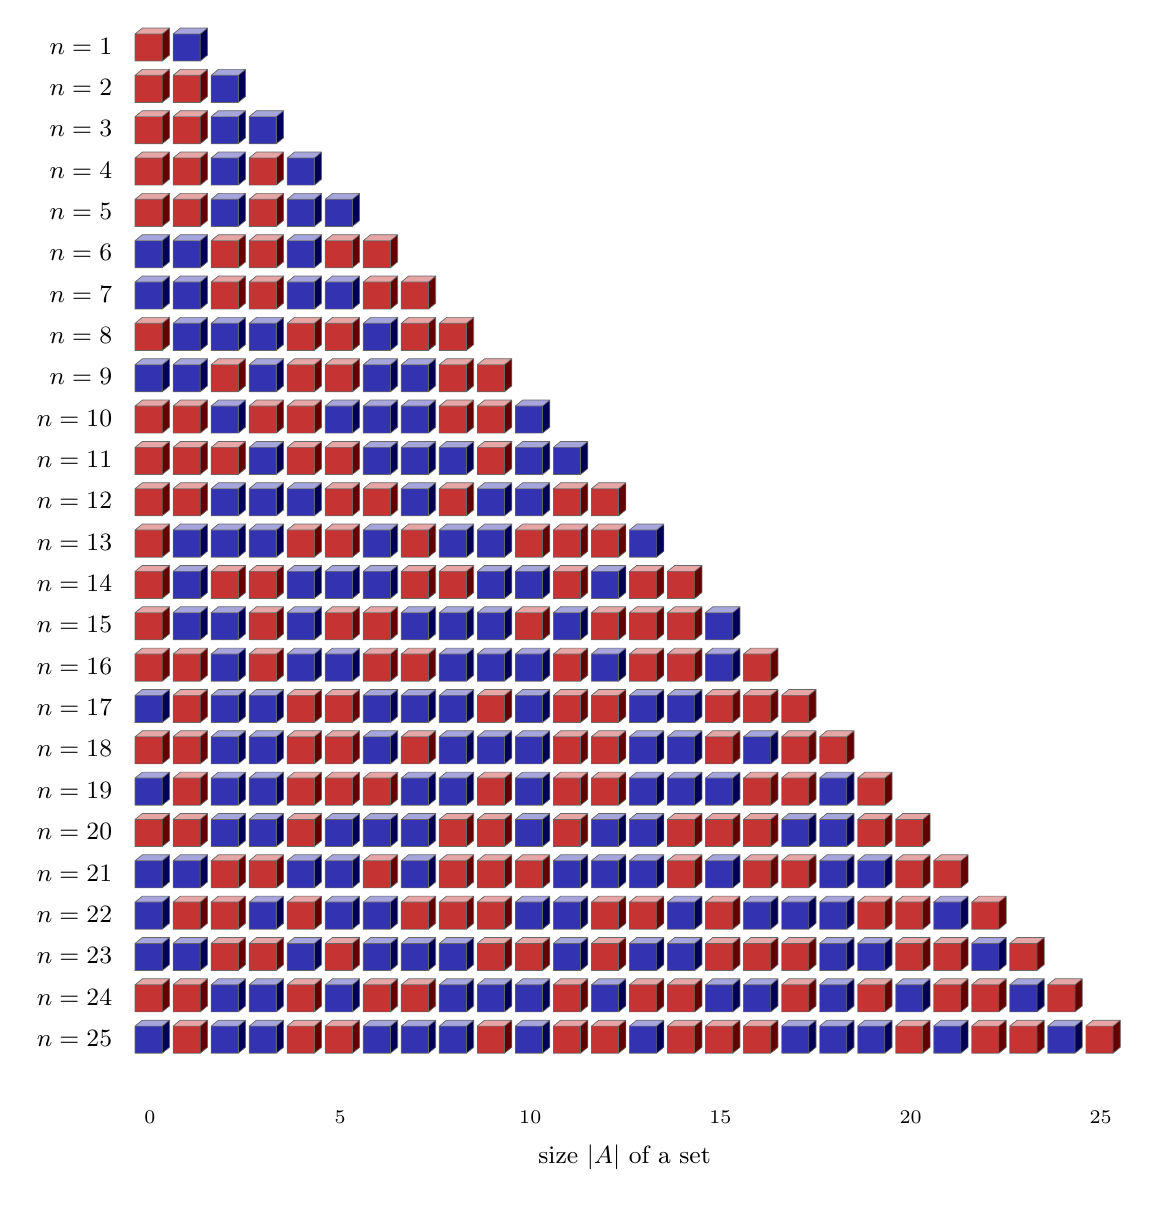
\begin{tikzpicture}[scale=0.42]
\foreach \n/\w in {
1/RB,2/RRB,3/RRBB,4/RRBRB,5/RRBRBB,6/BBRRBRR,7/BBRRBBRR,8/RBBBRRBRR,
9/BBRBRRBBRR,10/RRBRRBBBRRB,11/RRRBRRBBBRBB,12/RRBBBRRBRBBRR,13/RBBBRRBRBBRRRB,
14/RBRRBBBRRBBRBRR,15/RBBRBRRBBBRBRRRB,16/RRBRBBRRBBBRBRRBR,17/BRBBRRBBBRBRRBBRRR,
18/RRBBRRBRBBBRRBBRBRR,19/BRBBRRRBBRBRRBBBRRBR,20/RRBBRBBBRRBRBBRRRBBRR,
21/BBRRBBRBRRRBBBRBRRBBRR,22/BRRBRBBRRRBBRRBRBBBRRBR,23/BBRRBRBBBRRBRBBRRRBBRRBR,
24/RRBBRBRRBBBRBRRBBRBRBRRBR,25/BRBBRRBBBRBRRBRRRBBBRBRRBR}{
  \pgfmathsetmacro{\y}{-1.25*\n}
  \node[anchor=east,font=\small] at (-0.4,\y+0.45) {$n=\n$};
  \foreach \i in {0,...,\n}{
    \StrChar{\w}{\numexpr\i+1\relax}[\c]
    \if R\c \cube{1.15*\i}{\y}{cR}\else \cube{1.15*\i}{\y}{cB}\fi
  }
}
\foreach \i in {0,5,...,25}{\node[font=\scriptsize] at (1.15*\i+0.45,-33.2) {$\i$};}
\node[font=\small] at (14.8,-34.4) {size $|A|$ of a set};
\end{tikzpicture}
\end{document}
